\documentclass[11pt]{beamer}
\usepackage[utf8]{inputenc}
\usepackage{amsmath}
\usepackage{amsfonts}
\usepackage{amssymb}
\usepackage{graphicx}
\author{Lee Panter}
\title{Comparing Correlated Data Models on Single-Cell RNA Expression Profiles}
\date{Monday, November 25, 2019}

\begin{document}

\begin{frame}
\titlepage
\end{frame}


\begin{frame}{Presentation Overview}

\underline{Project Goals and Desired Outcomes:}
\begin{itemize}
	\item Develop multiple statistical models for Single-Cell RNA Sequencing data
	\item Compare the models for: fit, estimate stability, and diagnostic integrity.
	\item Suggest a model.  
\end{itemize}

\vspace{5pt}

\underline{Presentation Highlights:}
\begin{itemize}
	\item Introduction to RNA and Single-Cell
	\item Data Summaries and Proposed Modeling Approaches
	\item Results, Comparisons, and Conclusions
	\item Future Research, Outstanding Problems, Areas of Interest
\end{itemize}
\end{frame}

\begin{frame}{Introduction to RNA Sequencing}
	\underline{RNA Sequencing (RNAseq)}		
		\begin{itemize}
			\item Which genes are being expressed and at what magnitude?
			\item How do gene expressions change over time, or between treatment groups? \cite{maher2009transcriptome}	
			\item Used in: 
			\begin{itemize}
				\item Transcriptional Profiling
				\item Single Nucleotide Polymorphism (SNP) identification
				\item Differential Expression
			\end{itemize}
		\end{itemize}
	\underline{RNAseq Expression Profiles}
	\begin{itemize}
		\item Count data -- higher values $\Rightarrow$ higher level of expression
		\item Genes $\rightarrow$ (on/off)? $\Rightarrow$ Expression Value is $\ \left(  0 \ \ or \ \ > 0  \right)   \ $
		\item Indicative of zero-inflation
	\end{itemize}
\end{frame}


\begin{frame}{Single-Cell Methods}

\underline{Single-Cell (sc) Data:}
\begin{itemize}
	\item Measurements single-cell resolution
	\item \textit{Batch-Samples} from subjects $\Rightarrow$ Single-Cells ``sub-sampled" from each = Observational Units.
\end{itemize}

\vspace{5pt}

\underline{Repeated Measure/Clustering Assumptions:}
	\begin{itemize}
		\item SC observations are independent between Batch Samples
		\item Covariance between all Batch Samples assumed to be identical
	\end{itemize}

\vspace{5pt}

\underline{Case Study scRNA-seq Data:}
\begin{itemize}
	\item $\sim 38 * 10^{3}$ variables (genes), $\sim 9 * 10^3$ observations (SCs) 
	\item Poor measurement accuracy.  Problems with: batch effects, contamination, duplicate reads,...etc.
	\item Quality control filtering: $\sim 9 * 10^3$ obs $\longrightarrow$  $\sim 1,000$ obs \cite{SatijaLa52:online}
\end{itemize}
\end{frame}


%\begin{frame}{Motivating Example}
%\begin{figure}
%\centering
%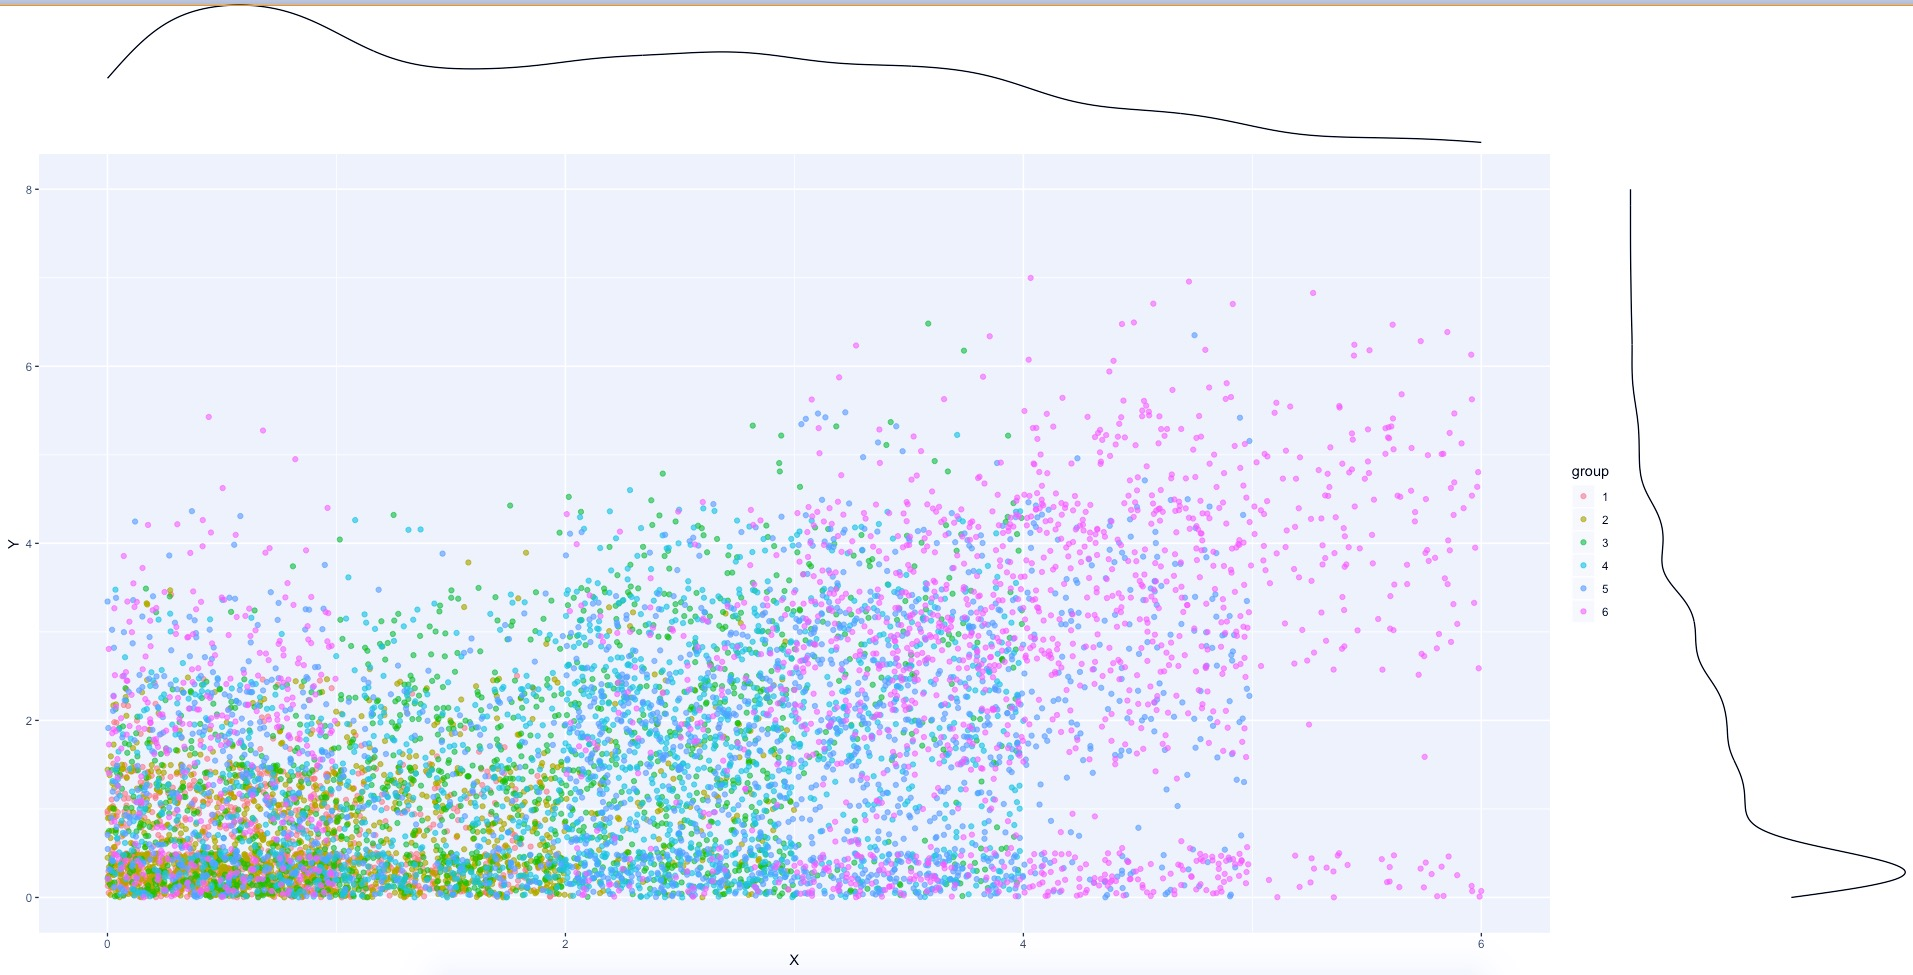
\includegraphics[width=1.07\textwidth]{2019-11-24_02-57-41.jpeg}
%\end{figure}
%\end{frame}
%
%
%\begin{frame}{Motivating Example}
%\begin{figure}
%\centering
%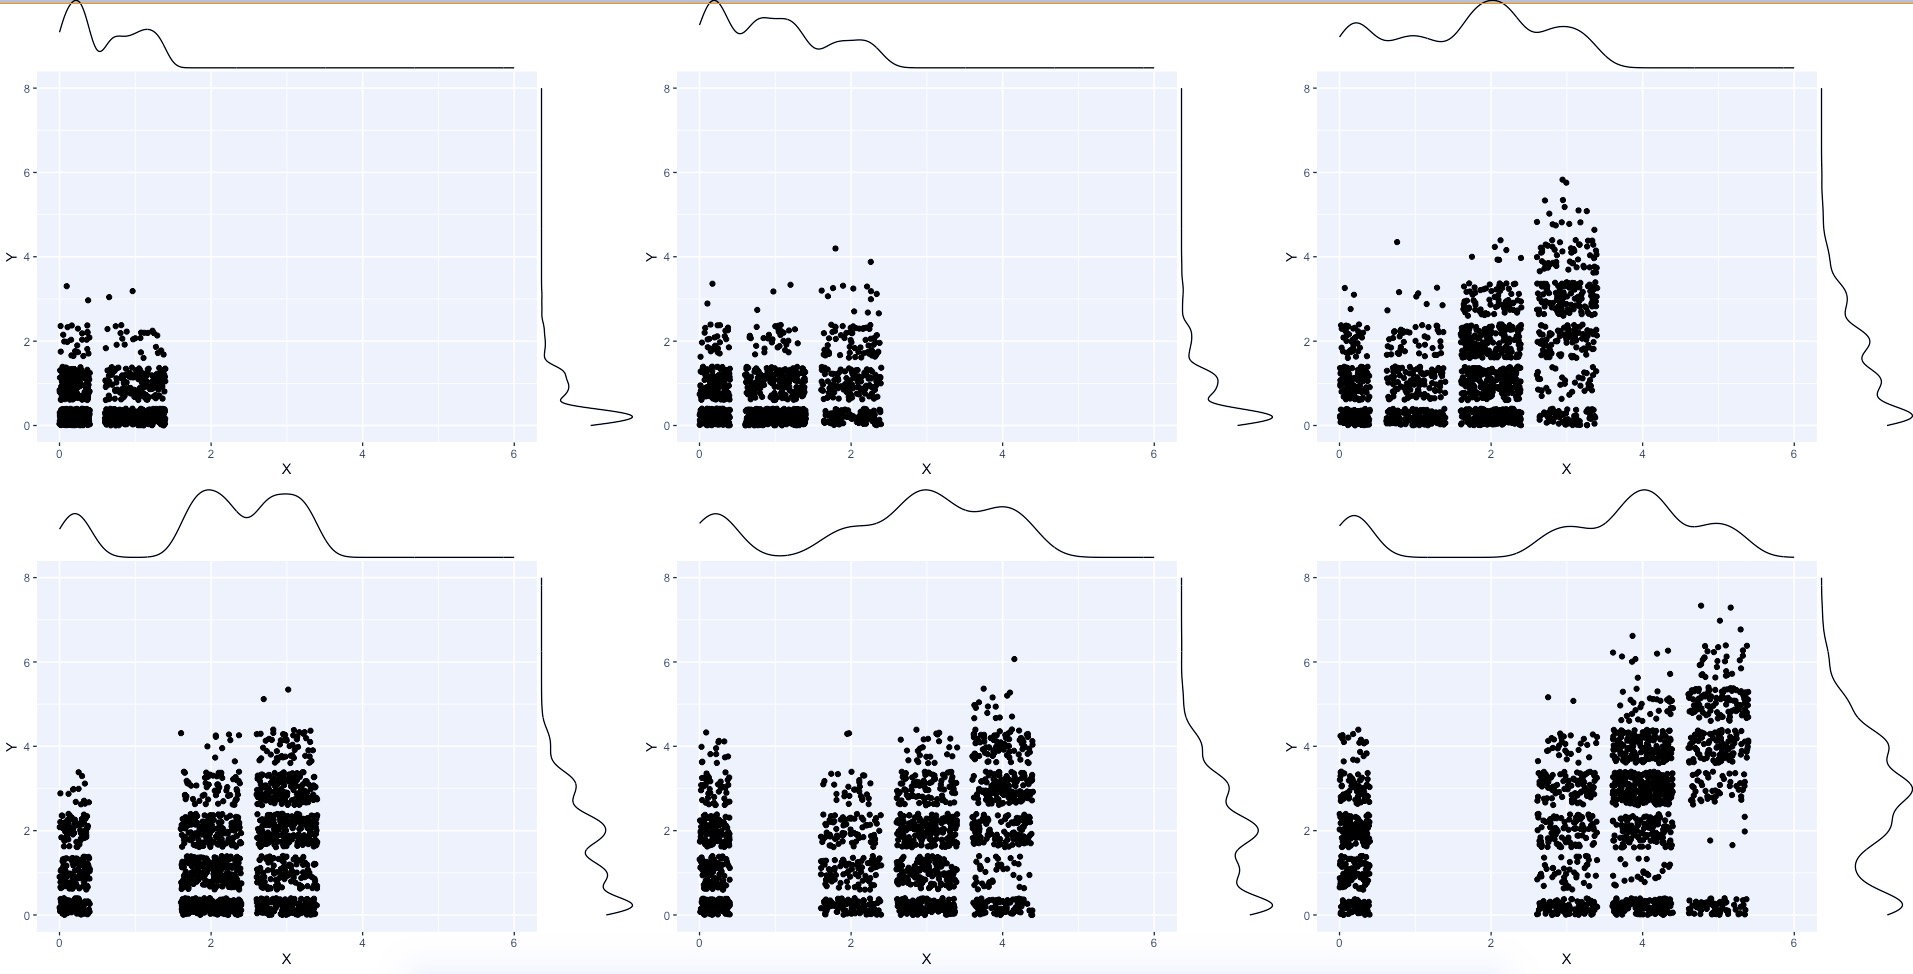
\includegraphics[width=1.07\textwidth]{2019-11-24_03-00-29.jpeg}
%\end{figure}
%\end{frame}


\begin{frame}{scRNA-seq Data Summary}
\begin{figure}
\centering
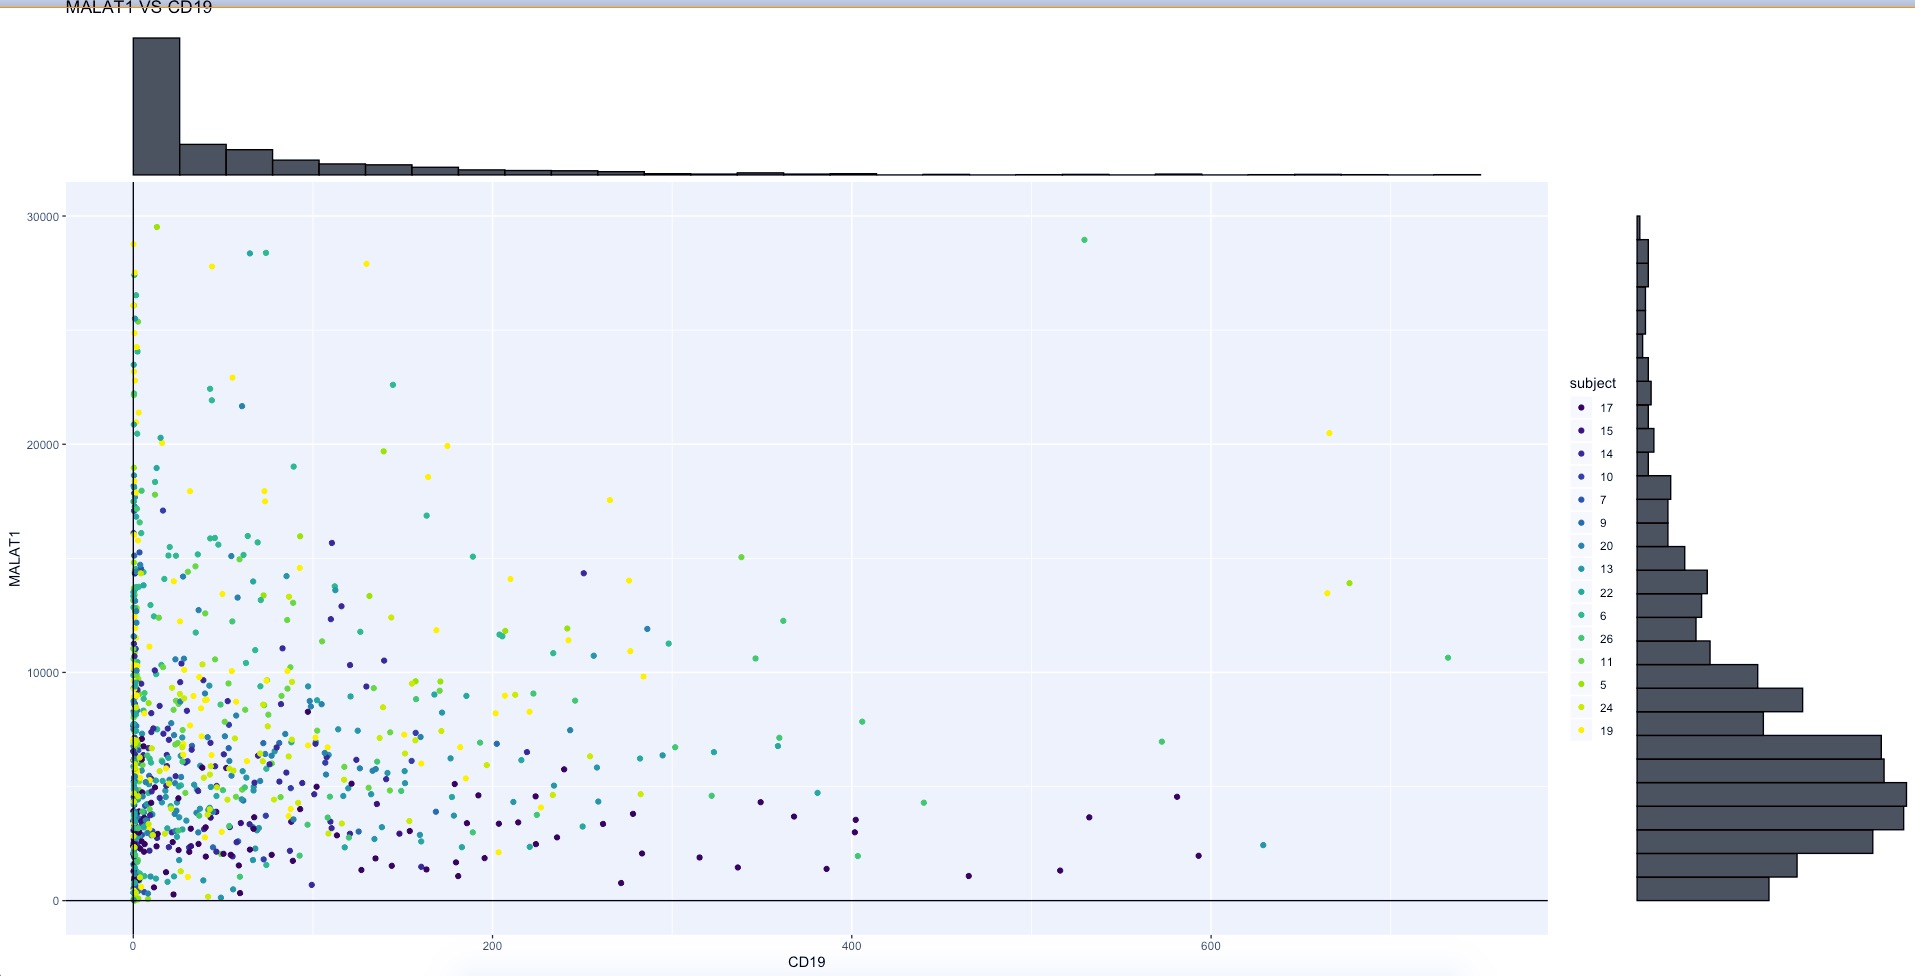
\includegraphics[width=1.07\textwidth]{2019-11-24_21-52-37.jpeg}
\caption{223 extreme observations removed to enlarge main distribution}
\end{figure}
\end{frame}


\begin{frame}{Proposed Modeling Approaches: Notation -- OLS \& LMM}

\begin{columns}



\begin{column}{0.47\textwidth}
\underline{Notation:}
		\vspace{5pt}
		\begin{itemize}
			\item Fixed Effects:
			\begin{itemize}
				\item[$\bullet$] Global Intercept:\\[0.5em] \hspace{5pt} $\sim 1+\cdots$\\[0.5em]
				\item[$\bullet$] Subject Factor: \\[0.5em] \hspace{5pt} $\sim subject+\cdots$\\[0.5em]
				\item[$\bullet$] Covariate Factor:\\[0.5em] \hspace{5pt}  $\sim CD19 +\cdots$\\[0.5em]
			\end{itemize}
			\item Random Effects:
			\begin{itemize}
				\item[$\bullet$] Intercept: \\[0.5em] \hspace{5pt} $\sim (1|subject)+\cdots$\\[0.5em]
				\item[$\bullet$] Slope:  \hspace{5pt} $\sim (CD19|subject) +\cdots$\\[0.5em]
			\end{itemize}
		\end{itemize}
\end{column}

\begin{column}{0.55\textwidth}
\vspace{5pt}
\underline{OLS and Linear Mixed Effects Models}
\begin{itemize}
		\setlength{\itemsep}{1\baselineskip}
	\item OLS:
	\begin{itemize}
			\setlength{\itemsep}{1\baselineskip}
		\item[$\bullet$] Predictors: \\
		$\sim$1 + CD19
	\end{itemize}
	\item LMM: 
	\begin{itemize}
			\setlength{\itemsep}{1\baselineskip}
		\item[$\bullet$] Fixed Effects:\\
		$\sim$ 1 + CD19
		\item[$\bullet$] Random Effects: \\
		 $\sim$ \footnotesize{(1 | subject) + (0 + CD19 | subject)}
		\item[$\bullet$] Repeated Measures: \\
		Unstructured (CS)
	\end{itemize}
\end{itemize}
\end{column}

\end{columns}

\end{frame}



\begin{frame}{Proposed Modeling Approaches: \small{Generalized Linear (Mixed) Models}}
\underline{Generalized Linear (Mixed) Models}
\vspace{5pt}
\begin{itemize}
	\item Poisson Regression (No Over-dispersion) \& Poisson Quasi-Likelihood (w/Over-dispersion)
	\vspace{5pt}
	\begin{itemize}
		\setlength{\itemsep}{1\baselineskip}
		\item[$\bullet$] Error Distribution: Poisson
		\item[$\bullet$] Linear Predictor: 1 + CD19
		\item[$\bullet$] Link Function: log
	\end{itemize}
	
	\vspace{5pt}
	
	\item Generalized Linear Mixed Models (Penalized QL)
	\vspace{5pt}
	\begin{itemize}
	\setlength{\itemsep}{1\baselineskip}
		\item[$\bullet$] Error Distribution: Poisson
		\item[$\bullet$] Linear Predictor(s):\\
		 FIXED=1 + CD19\\
		 RANDOM=(1 | subject) + (0 + CD19 | subject)
		\item[$\bullet$] Link Function: log
	\end{itemize}
\end{itemize}
\end{frame}


\begin{frame}{Proposed Modeling Approaches: Zero Inflated Poisson}

\textbf{Occurrence Model:} $R_{ij} \sim bernoulli \left( p_{ij} | a_{0}, a_{1}  \right)$\\

where $a_{0}, a_{1}$ are \underline{Occurrence-Model} random effect parameters\\

\vspace{10pt}

\textbf{Intensity Model:} $Y_{ij} | \left( r_{ij}=1, a_{0}, a_{1}  \right),  \sim Poisson \left( \lambda_{ij} | b_{0}, b_{1}  \right) $\\
 where $b_{0}, b_{1}$ are \underline{Intensity-Model} random effect parameters\\

\vspace{10pt}

\textbf{Zero-Inflated Poisson, Generalized Linear (Mixed) Models}\\
\vspace{5pt}
\textit{Fit Using Adaptive Gauss-Hermite Quadrature}\\

\vspace{5pt}

	\begin{itemize}
		\setlength{\itemsep}{1\baselineskip}
		\item[$\bullet$] Error Distribution: ``Zero-Inflated Poisson"
		\item[$\bullet$] Occurence \& Intensity Model Linear Predictors: 
		\begin{itemize}
			\item[$\circ$] Fixed Effects: $\left \{   \sim 1, \sim 1+CD19  \right \}$
			\item[$\circ$] Random Effects: $\left \{   \sim 1, \sim 1+CD19  \right \}$
		\end{itemize}
		\item[$\bullet$] Link Function: Log
	\end{itemize}
\end{frame}


\begin{frame}{Results, Comparisons, Conclusions}

\begin{center}
\begin{tabular}{|c||c|c|c|}
\hline
Model	 &	 Intercept Estimate	&	Std.Err	&	p-value \\
\hline
\hline
LMwFE &  $7.7624 * 10^{3}$ &  $2.3480 * 10^{2}$ & $< 2 * 10^{-16}$  \\
\hline
LMMwRE & $7.338 * 10^{3}$& $7.6776* 10^{2}$ & $< 2 * 10^{-16}$ \\
\hline
POI & 8.957 & $ 3.723 * 10^{-4}$ & $< 2 * 10^{-16}$  \\
\hline
POIql & 8.957 & $3.007 * 10^{-2}$ & $< 2 * 10^{-16}$  \\
\hline
POIqlLMM & 8.8362 & $1.0160* 10^{-1}$ &  $1.7* 10^{-3}$ \\
\hline
ZIP & 8.9572 & $< 2 * 10^{-4}$ & $< 2 * 10^{-4}$ \\
\hline
\end{tabular}
\end{center}


\begin{center}
\begin{tabular}{|c||c|c|c|}
\hline
Model	 &	 Slope Estimate	&	Std.Err	&	p-value \\
\hline
\hline
LMwFE & $7.1320* 10^{-1}$ & 1.5426 &  $6.440* 10^{-1}$  \\
\hline
LMMwRE  & 2.168 & 1.797 & $2.278* 10^{-1}$ \\
\hline
POI & $8.839 * 10^{-5}$ & $2.369 * 10^{-6}$ & $< 2 * 10^{-16}$ \\
\hline
POIql  & $8.839 * 10^{-5}$ & $1.913 * 10^{-4}$ & $6.440* 10^{-1}$ \\
\hline
POIqlLMM  & $3.16* 10^{-4}$ &  $1.653* 10^{-4}$ &  $5.61* 10^{-2}$\\
\hline
ZIP & $1* 10^{-4}$& $2.03 * 10^{-6}$ & $< 2 * 10^{-16}$ \\
\hline
\end{tabular}
\end{center}
Note: $e^{8.957} \approx 7.762 * 10^{3}$
\end{frame}



\begin{frame}{Results, Comparisons, Conclusions}

\begin{columns}

\begin{column}{0.5\textwidth}
\underline{\textbf{Conclusions Drawn from Results:}}
\begin{itemize}
	\item Simpler models performed better according to the AIC criterion\\[1em]
	\item Parameter estimates for global intercept showed higher stability and significance than estimates for  slope
\end{itemize}
\end{column}

\begin{column}{0.5\textwidth}
\centering
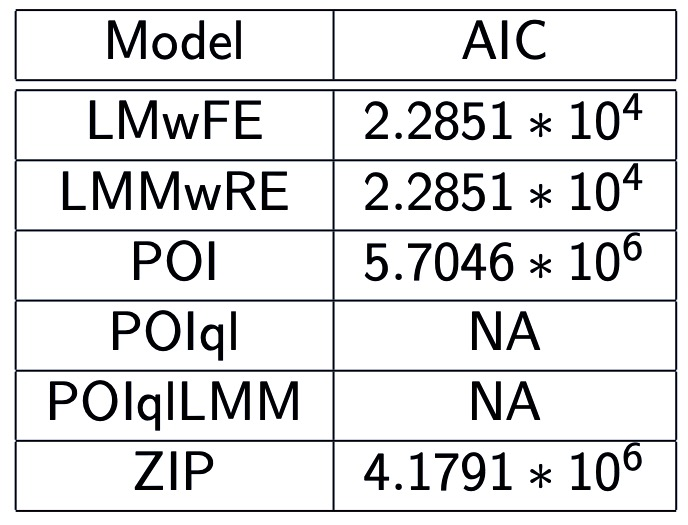
\includegraphics[width=\textwidth]{2019-11-25_03-05-00.jpeg}
\end{column}
\end{columns}
\end{frame}


\begin{frame}{Future Research, Outstanding Problems, Areas of Interest}

\textbf{\underline{Outstanding Issues:}}
\begin{itemize}
	\item Comparing quasi-likelihood models to linear models and quadrature methods
\end{itemize}

\vspace{5pt}

\textbf{\underline{Future Research \& Areas of Interest:}}
\begin{itemize}
	\item Log-transformed responses, additional variable combinations, marginal average models
\end{itemize}

\vspace{15pt}

\begin{center}
\Large{\textbf{\underline{Thanks for Listening!}}}
\end{center}

\end{frame}



\section{References}

\begin{frame}[allowframebreaks]{References}
\bibliographystyle{unsrt}
\bibliography{PresentBib}
\end{frame}




\end{document}